\documentclass[final]{beamer}
%\usepackage{etex}

\usetheme{boxes}
\usecolortheme{rose}
\usefonttheme{professionalfonts}
%\setbeamertemplate{mini frames}{}
\usepackage[english]{babel}
\usepackage[utf8]{inputenc}
\usepackage[T1]{fontenc}
\usepackage{amsfonts,amssymb,amsmath}
\usepackage{esint}
%\usepackage{epstopdf}
\usepackage{algorithmic}
% \usepackage{algorithm}
\usepackage{tikz}
\usetikzlibrary{arrows,shapes}
%\usepackage{xifthen}
\usepackage{pgfplots}
\usepackage{float}
\usepackage{ragged2e}
%\usepackage{latexsym}
%\usepackage[dvips]{pstricks} % PSTricks
%\usepackage{pst-node}
%\usepackage{psfrag}
%\usepackage{wrapfig}
%\usepackage{alltt}
%\usepackage{url}
%\usepackage{pict2e}
%\usepackage{multimedia}
%\usepackage{fancyvrb}
\usepackage{graphicx}
%\usepackage{verbatim}
%\usepackage{mathrsfs}
%\usepackage{multirow}
\usepackage{bm}
%\usepackage{algorithm2e}
\usepackage{hyperref}
%\usepackage[angle=0,scale=5,opacity=1,color=black]{background}
%\usepackage[active]{srcltx}
\usepackage{commath}
\usepackage{multicol}
%\usepackage[export]{adjustbox}


%\usetikzlibrary{spy}
%\tikzset{level 1 concept/.append style={font=\sf, sibling angle=60,level distance = 27mm}}
%\tikzset{level 2 concept/.append style={font=\sf, sibling angle=55,level distance = 17mm}}
%\tikzset{every node/.append style={scale=0.6}} 


%% Beamer Style Setup
%\definecolor{mywine}{rgb}{.5412,.0235,.0}
%\usecolortheme[named=mywine]{structure}
%\setbeamercolor{title}{fg=mywine}
%\setbeamercolor{frametitle}{fg=mywine}
%\setbeamercovered{transparent}
\setbeamertemplate{navigation symbols}{}

%% ALGORITHM Commands %%%%%%%%%%%%%%%%%%%%%%%%%%%%%%
\renewcommand{\algorithmicrequire}{\textbf{Input:}}
\renewcommand{\algorithmicensure}{\textbf{Output:}}
\newfloat{program}{thp}{Program}
\floatname{program}{}
\renewcommand*\theprogram{}
\newcommand{\theHalgorithm}{\arabic{algorithm}}
\newcommand{\eq}[1]{(\ref{#1})}




\newtheorem{remark}[theorem]{Remark}
\newtheorem{proposition}[theorem]{Proposition}


\renewcommand{\Im}{{\ensuremath{\mathrm{Im\,}}}}
\renewcommand{\Re}{{\ensuremath{\mathrm{Re\,}}}}

\newcommand{\R}{\mathbb{R}}
\newcommand{\C}{\mathbb{C}}
\newcommand{\N}{\mathbb{N}}

\setbeamertemplate{caption}[numbered]

\selectlanguage{english}
\title[SIMP Optimization]{\bf Topological Optimization Using the SIMP Method}
\author[Mikal Nelson]{Mikal Nelson
%(joint work with XXXXX) 
}
\institute[KU]{
{University of Kansas}\\
Department of Mathematics\\
mikal.nelson@ku.edu\\
}
\date[M.A. Thesis Defense]{
\small M.A. Thesis Defense\\
July 26\textsuperscript{th}, 2021\\
Zoom
}
\titlegraphic{\hspace{0in}
\includegraphics[scale=0.35]{logos/ku_math_logo.png}\;
\hspace{1.2in}
\includegraphics[scale=0.12]{logos/ku_logo}\;

}

\graphicspath{ {pictures/} }

\begin{document}

\frame{
\titlepage
}

\frame{
	
	\structure{\bf Outline}
	
	\medskip
	\begin{itemize}
		\item Heat Equation and Finite Volume Method
		\item Optimization and Method of Moving Asymptotes
		\item Solid Isotropic Material with Penalization (SIMP)
		\item Algorithm Results
	\end{itemize}
	%
	
}

\frame{

\structure{\bf Heat Equation}

\medskip
The temperature ($T$) at any point in such an object is a function of both space ($\mathbf{x}$) and time ($t$) coordinates: $T(\mathbf{x},t)$.\\\vspace{1em}
Physical principles demand that such a temperature function must satisfy the equation
\begin{equation}
	\frac{\partial T}{\partial t}=\nabla\cdot\left(k(\mathbf{x})\nabla T\right)\label{eqn:HeatEq},
\end{equation}
where $\nabla$ is the gradient operator and the function $k$ represents the thermal diffusivity at a point in our object.
%

}
\begin{frame}
	\begin{figure}
		\centering
		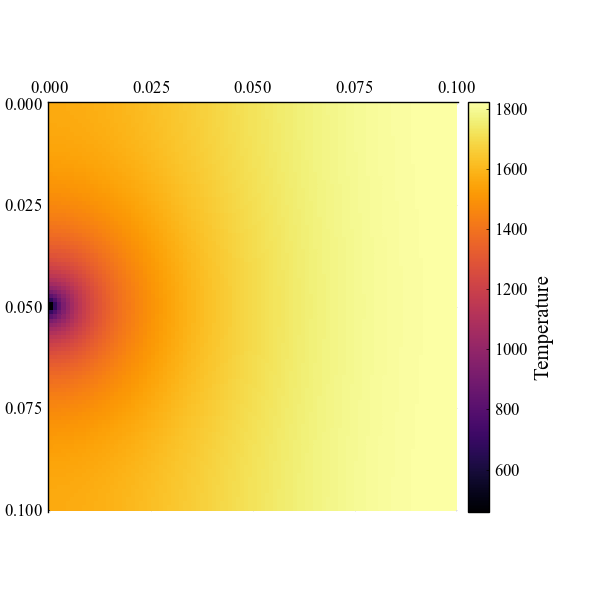
\includegraphics[width=0.65\textwidth]{Heatmap_Example.png}
		\caption[Heatmap Example]{Heatmap for a 0.1m $\times$ 0.1m object with uniform heat generation and a heat sink at the center of its west boundary. This map was produced via the Finite Volume Method using $100\times 100$ uniform control volumes.}
		\label{fig:heatmap-example}
	\end{figure}
\end{frame}

\begin{frame}
	\structure{\bf Finite Volume Method (FVM)}
\end{frame}

\begin{frame}
	\begin{theorem}[The Divergence Theorem]
		Suppose that $\mathcal{V}$ is a compact subset of $\mathbb{R}^n$ that has a piecewise smooth boundary $\mathcal{S}$ (i.e. $\partial\mathcal{V}=\mathcal{S}$) with outward pointing normal vectors. If $\mathbf{F}$ is a continously differentiable vector field defined on a neighborhood of $\mathcal{V}$, then
		\begin{equation}
			\iiint_{\mathcal{V}}\left(\nabla\cdot\mathbf{F}\right)\dif\mathcal{V}=\oiint_{\mathcal{S}}\left(\mathbf{F}\cdot\mathbf{\hat{n}}\right)\dif\mathcal{S}\label{eqn:div-thm}
		\end{equation}
		where $\hat{n}$ is the outwards pointing normal vector to the boundary.
		\label{thm:div-thm}
	\end{theorem}
\end{frame}

\begin{frame}
	\structure{\bf Discretization of Heat Equation}
	\begin{equation}
		\int_{V_i}\frac{\partial T}{\partial t}\dif\mathbf{x}=\int_{V_i}\nabla\cdot \left(k(\mathbf{x})\nabla T\right)\dif\mathbf{x}\underset{\eqref{eqn:div-thm}}{=}\int_{\partial V_i}k(\mathbf{x})\nabla T\cdot\hat{\mathbf{n}}\dif s\label{eqn:Vol-to-Surface-FVM}
	\end{equation}\\
	\vspace{1em}
	In a square grid there are only four neighboring cells which we can label as North, South, East, West.\\\vspace{1em}
	For a control volume $V_i$ we'll label the North boundary as $\partial V_N$, the South boundary as $\partial V_S$, the East boundary as $\partial V_E$, and the West boundary as $\partial V_W$.\\\vspace{1em}
	Additionally, let $\Delta x$ be the length of the North and South boundaries, and $\Delta y$ the length of the East and West boundaries.
\end{frame}

\begin{frame}
	\structure{\bf Discretization of Heat Equation}
	\begin{equation*}
		\int_{V_i}\frac{\partial T}{\partial t}\dif\mathbf{x}=\int_{V_i}\nabla\cdot \left(k(\mathbf{x})\nabla T\right)\dif\mathbf{x}\underset{\eqref{eqn:div-thm}}{=}\int_{\partial V_i}k(\mathbf{x})\nabla T\cdot\hat{\mathbf{n}}\dif s
	\end{equation*}
	\hspace*{-2pt}\makebox[\linewidth][c]{%
	\begin{tabular}{ccc}
		$\displaystyle\int_{\partial V_i}k(\mathbf{x})\nabla T\cdot\hat{\mathbf{n}}\dif s$ & $=$ & $\displaystyle\int_{\partial V_N}k(\mathbf{x})\nabla T\cdot\hat{\mathbf{n}}_N\dif s+\int_{\partial V_S}k(\mathbf{x})\nabla T\cdot\hat{\mathbf{n}}_S\dif s$\\
		&  & $\displaystyle+\int_{\partial V_E}k(\mathbf{x})\nabla T\cdot\hat{\mathbf{n}}_E\dif s+\int_{\partial V_W}k(\mathbf{x})\nabla T\cdot\hat{\mathbf{n}}_W\dif s$
	\end{tabular}
	}
\end{frame}

\begin{frame}
	\hspace*{-2pt}\makebox[\linewidth][c]{%
			\begin{tabular}{ccc}
				$\displaystyle\int_{\partial V_i}k(\mathbf{x})\nabla T\cdot\hat{\mathbf{n}}\dif s$ & $=$ & $\displaystyle\int_{\partial V_N}k(\mathbf{x})\nabla T\cdot\hat{\mathbf{n}}_N\dif s+\int_{\partial V_S}k(\mathbf{x})\nabla T\cdot\hat{\mathbf{n}}_S\dif s$\\
				&  & $\displaystyle+\int_{\partial V_E}k(\mathbf{x})\nabla T\cdot\hat{\mathbf{n}}_E\dif s+\int_{\partial V_W}k(\mathbf{x})\nabla T\cdot\hat{\mathbf{n}}_W\dif s$
			\end{tabular}
	}
\end{frame}

\begin{frame}
	\hspace*{-2pt}\makebox[\linewidth][c]{%
		\begin{tabular}{ccc}
			$\displaystyle\int_{\partial V_i}k(\mathbf{x})\nabla T\cdot\hat{\mathbf{n}}\dif s$ & $=$ & $\displaystyle\int_{\partial V_N}k(\mathbf{x})\nabla T\cdot\hat{\mathbf{n}}_N\dif s+\int_{\partial V_S}k(\mathbf{x})\nabla T\cdot\hat{\mathbf{n}}_S\dif s$\\
			&  & $\displaystyle+\int_{\partial V_E}k(\mathbf{x})\nabla T\cdot\hat{\mathbf{n}}_E\dif s+\int_{\partial V_W}k(\mathbf{x})\nabla T\cdot\hat{\mathbf{n}}_W\dif s$\\
			& & \\
			$\displaystyle\int_{V_i}\frac{\partial T}{\partial t}\dif\mathbf{x}$ & $\approx$ & $\displaystyle k_N\frac{T_N-T_i}{\|\mathbf{x}_N-\mathbf{x}_i\|}\Delta y+k_S\frac{T_S-T_i}{\|\mathbf{x}_S-\mathbf{x}_i\|}\Delta y$\\
			& & $\displaystyle+k_E\frac{T_E-T_i}{\|\mathbf{x}_E-\mathbf{x}_i\|}\Delta x+k_W\frac{T_W-T_i}{\|\mathbf{x}_W-\mathbf{x}_i\|}\Delta x$
		\end{tabular}
	}
\end{frame}

\begin{frame}
	\hspace*{-2pt}\makebox[\linewidth][c]{%
		\begin{tabular}{ccc}
			$\displaystyle\int_{\partial V_i}k(\mathbf{x})\nabla T\cdot\hat{\mathbf{n}}\dif s$ & $=$ & $\displaystyle\int_{\partial V_N}k(\mathbf{x})\nabla T\cdot\hat{\mathbf{n}}_N\dif s+\int_{\partial V_S}k(\mathbf{x})\nabla T\cdot\hat{\mathbf{n}}_S\dif s$\\
			&  & $\displaystyle+\int_{\partial V_E}k(\mathbf{x})\nabla T\cdot\hat{\mathbf{n}}_E\dif s+\int_{\partial V_W}k(\mathbf{x})\nabla T\cdot\hat{\mathbf{n}}_W\dif s$\\
			& & \\
			$\displaystyle\int_{V_i}\frac{\partial T}{\partial t}\dif\mathbf{x}$ & $\approx$ & $\displaystyle k_N\frac{T_N-T_i}{\|\mathbf{x}_N-\mathbf{x}_i\|}\Delta y+k_S\frac{T_S-T_i}{\|\mathbf{x}_S-\mathbf{x}_i\|}\Delta y$\\
			& & $\displaystyle+k_E\frac{T_E-T_i}{\|\mathbf{x}_E-\mathbf{x}_i\|}\Delta x+k_W\frac{T_W-T_i}{\|\mathbf{x}_W-\mathbf{x}_i\|}\Delta x$\\
			& & \\
			$\displaystyle\implies \Delta x\Delta y\frac{\dif T_i}{\dif t}$ & $=$ & $\displaystyle\left( k_N\frac{T_N-T_i}{\|\mathbf{x}_N-\mathbf{x}_i\|}+k_S\frac{T_S-T_i}{\|\mathbf{x}_S-\mathbf{x}_i\|}\right)\Delta y$\\
			& & $\displaystyle+\left(k_E\frac{T_E-T_i}{\|\mathbf{x}_E-\mathbf{x}_i\|}+k_W\frac{T_W-T_i}{\|\mathbf{x}_W-\mathbf{x}_i\|}\right)\Delta x$
		\end{tabular}\label{deriv:descrete-FVM}
	}
\end{frame}

\frame[plain,allowframebreaks]{
\structure{\bf Bibliography}

\medskip
\begin{tiny}
\bibliographystyle{plain}
\bibliography{Thesis_Bibliography.bib}
\nocite{Boyd2004}
\nocite{Gander2018}
\nocite{Marck2012}
\nocite{Svanberg1987}
\nocite{Versteeg2007}
\end{tiny}
}

\end{document}
 
